\section{Partes de un mapa mental.}

\subsection{Según su estructura.}
Un mapa mental tiene las siguientes estructuras esenciales (figura \ref{fig:partesestructura}):

\begin{enumerate}
\item Idea central.
\item Aristas. Establece una asociación de ideas.
\item Nodo. Ideas segundarías o asociada a otra idea.
\end{enumerate}

\begin{figure}[htbp]
\centering
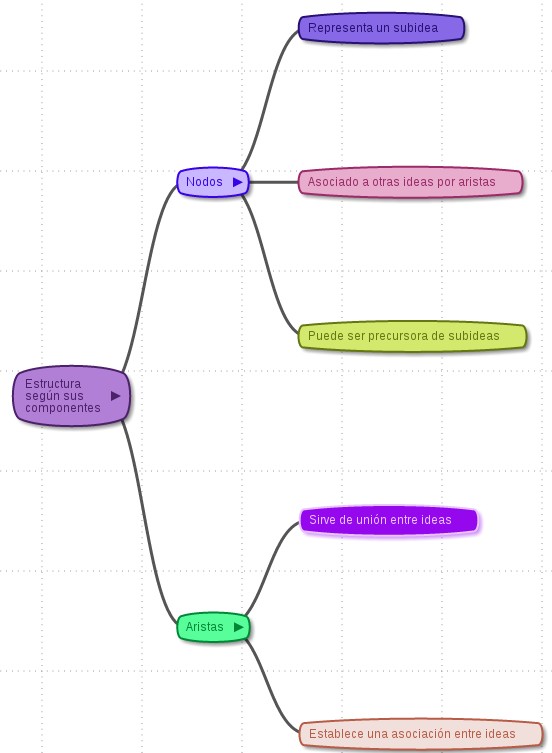
\includegraphics[width=0.6\textwidth]{imagenes/Estructura2.png}
\caption{Partes de un mapa mental}
\label{fig:partesestructura}
\end{figure}

\subsection{Por contenido.}

Un mapa mental podemos estructurarlo según su contenido (figura \ref{fig:partescontenido}).

\begin{enumerate}
\item Idea central
\item Los temas principales del asunto irradian de la imagen central como ramas.
\item Cada rama contiene una imagen o una palabra clave asociada.
\item Las ramas forman una estructura nodal conectada.
\end{enumerate}

\begin{figure}[htbp]
\centering
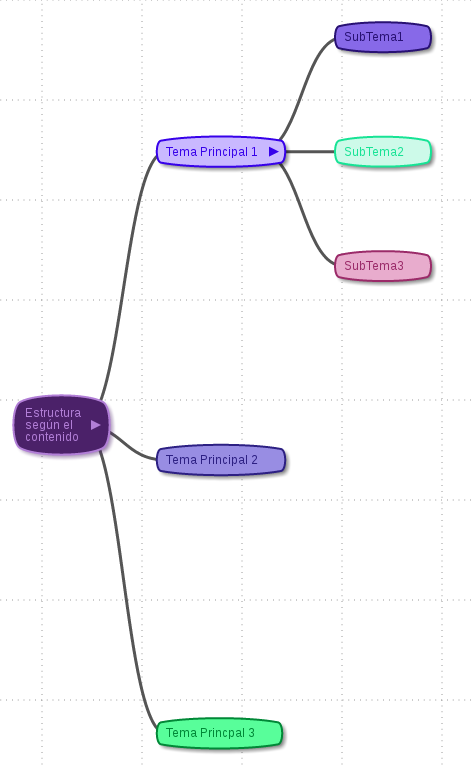
\includegraphics[width=0.6\textwidth]{imagenes/Estructura1.png}
\caption{Partes de un mapa mental considerando su contenido}
\label{fig:partescontenido}
\end{figure}